%Correct the file name.
%X: book number
%Y: part number
%ZZZ: page number in three digits. So page 3 would be 003.

\documentclass[11pt]{amsbook}

\usepackage{../HBSuerDemir}	% ------------------------

\begin{document}

% ++++++++++++++++++++++++++++++++++++++
\hPage{b2p1/213}
% ++++++++++++++++++++++++++++++++++++++

\noindent b) the ellipsoid $4x^2+y^2+z^2=16$

\begin{hSolution}
 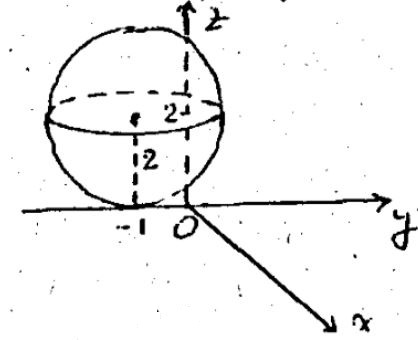
\includegraphics[width=0.45\textwidth]{images/b2p1-213-fig01}\\
a) The center is at $\hPairingParan{-1,0,2}$ and radius is equal to $2$. \\
 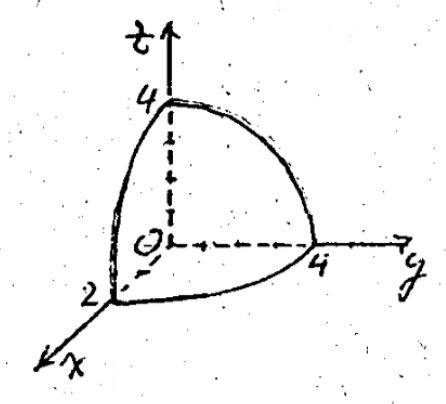
\includegraphics[width=0.45\textwidth]{images/b2p1-213-fig02}\\
b) Writing it in the form
$$
\frac{x^2}{2^2}+\frac{y^2}{4^2}+\frac{z^2}{4^2}=1
$$
one has $a=2$, $b=4$, $c=4$ and that part in the I. octant is shown in the figure. 

\end{hSolution}

\begin{exmp}
Sketch the quadrics:\\

\begin{tabular}{ll}
a) $\frac{x^2}{4}-\frac{y^2}{9}-\frac{z^2}{4}=1$\quad \quad \quad \quad 
b)  $\frac{x^2}{4}-z^2=2y$
\end{tabular}
\begin{hSolution}
 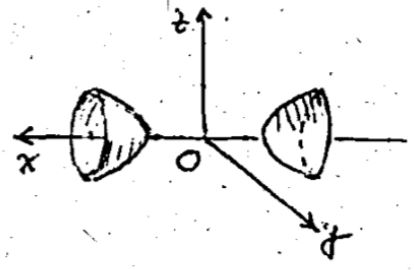
\includegraphics[width=0.45\textwidth]{images/b2p1-213-fig03}\\
a) The surface is a hyperboloid of two sheets with semi axes $a=2$, $b=3$, $c=2$ admitting $0x$ as axis. Cross sections // yz-plane cease to exist when $-2<x<2$.\\
 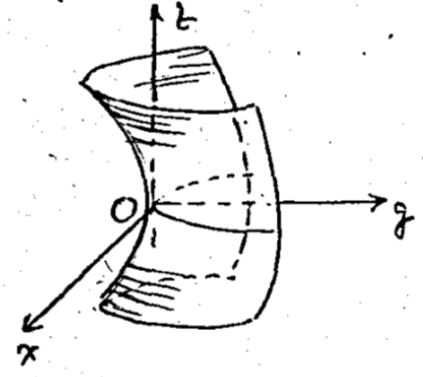
\includegraphics[width=0.45\textwidth]{images/b2p1-213-fig04}\\
b)The surface is a hyperbolic paraboloid (or a saddle shaped surface).\\
$x=0 \implies y=-\frac{z^2}{2}$ (a parabola)\\
$z=0 \implies y=x^2/8$ (a parabola)
 
\end{hSolution}
\end{exmp}
\section*{E. SECOND DEGREE SURFACES}
The quadrics being second degree surfaces, their equations are included in the general equation 
\end{document}  